\section{Design}
The design of the robot is done with the 3D design software \href{https://www.freecadweb.org/}{Free-cad}. All part files are uploaded to the GitHub repository \url{https://github.com/tarragoesteve/TFM} under the hardware folder.

You can see the main views on Figure \ref{fig:Isometric render view}, \ref{fig:Front render view}, \ref{fig:Top render view} and \ref{fig:Side render view}.

We included three actuators in the robot because we want to control three degrees of freedom (inclination and speed of both wheels). Furthermore we introduced a fly-wheel/pendulum so we can control the inclination of the body. 

We ensured symmetry along the axis formed by all motors in order to have an equilibrium in all possible inclinations without the need of external forces. We also took in consideration that the reinforcement learning algorithm starts being clumsy so none of the configurations should intersect with the ground. Figure \ref{fig:Side render view} illustrates this restriction.   

\begin{figure}
	\centering
	\includegraphics[width=10cm]{img/isometric_view.png}
	\caption{Isometric render view}
	\label{fig:Isometric render view}
\end{figure}
\begin{figure}
	\centering
	\includegraphics[width=10cm]{img/front_view.png}
	\caption{Front render view}
	\label{fig:Front render view}
\end{figure}
\begin{figure}
	\centering
	\includegraphics[width=10cm]{img/top_view.png}
	\caption{Top render view}
	\label{fig:Top render view}
\end{figure}
\begin{figure}
	\centering
	\includegraphics[width=4cm]{img/side_view.png}
	\caption{Side render view}
	\label{fig:Side render view}
\end{figure}

\subsection{Flywheel design}
\begin{figure}
	\centering
	\includegraphics[width=5cm]{img/fly_wheel_side.png}
	\caption{Fly wheel side render view}
	\label{fig:Fly wheel side render view}
\end{figure}

To control the inclination of the body two strategies are taken in to account. Creating torque by a pendulum or accelerating the flywheel. In order to experiment with both of them we designed a part to allow both configuration by placing weights in different spots, see figure \ref{fig:Fly wheel side render view}.

In order to create a configuration with maximum gravitational torque we have done the following computation. We denote the torque pendulum torque $\tau$, consider the masses are cylinders of mass $m_{cylinder}$ with radius $r_c$ and width $w$ and the radius of the flywheel is $r_f$.

Each mass weights:
\[ m_{cylinder} = \rho * w * \pi * r_c^2 \]

We will neglect the mass of the flywheel structure versus the mass of the cylinders.

All the gravitational torque created by the masses will be compensated with the opposite weight except for the two masses with different radius.

One of the weight can be placed along a rail. The distance to the center will vary from $r_{min} = r_c + r_{motor-axis} \approx r_c $ to $r_{max} = r_f - r_c$. 

The maximum torque takes place when these two masses are aligned horizontal with respect the ground and the movable weight is at distance $r_{min}$ from the center.

\[ \tau _{max} (r_c) =  m_{cylinder} * g * r_{max} -  m_{cylinder} * g * r_{min} =  m_{cylinder}* g * (r_f - 2 * r_c) \]

In order to maximize $\tau$ it we first compute the derivative:
\[\frac{\partial \tau _{max} (r_c)}{\partial r_c} = g *(\frac{\partial m}{\partial r_c} * (r_f - 2 * r_c) -  m_{cylinder} * 2)\]

\[ \frac{\partial  m_{cylinder}}{\partial r_c} = 2 * \rho * w * \pi *  r_c\]

An make it zero to find the maximum:

\[\frac{\partial \tau _{max} (r_c)}{\partial r_c} = 0\]

Substituting and simplifying we get:

\[\frac{\partial m}{\partial r_c} * (r_f - 2 * r_c) =   m_{cylinder} * 2 \Rightarrow 2 * \rho * w * \pi *  r_c\ * (r_f - 2 * r_c) = \rho * w * \pi * r_c^2 * 2 \]

\[ \Rightarrow r_c\ * (r_f - 2 * r_c) =  r_c^2 \Rightarrow (r_f - 2 * r_c) =  r_c \Rightarrow \boxed{r_f = 3 * r_c}\]


The circumradius $R$ from the center of a regular polygon to one of the vertices is related to the side length $s$ by:

\begin{center}
	\begin{tabular}{ c  c }
		\(\displaystyle R=\frac {s}{2* \sin{\frac {\pi} {n}}} \)
		& 
		\includegraphics[width=3cm]{img/PolygonParameters.png}
	\end{tabular}
\end{center}

In our case:
\[ R = r_f - r_c; \]
\[ s = 2 * r_c\]

Substituting in the circumradius equation we get n = 6, so we will use up 6 masses in our flywheel.
We will have a variable number of masses $N$ that we will be able to add to the flywheel as shown in the following table.
\begin{center}
	\begin{tabular}{c | c | c | c }
	 2 & 3 & 4 & 6 \\
	 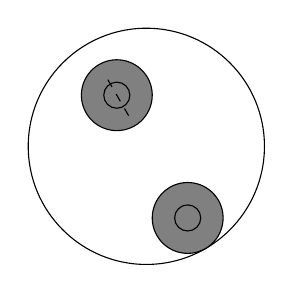
\begin{tikzpicture}[scale=0.5]
		%Circle
			\path node (center) at (0,0) {};
			\draw (center) circle (3);
		%Movable mass
			\draw[rotate=120,fill=gray] (1.5,0) circle (.9) node (moving) [draw,circle]{};
		%Guide
			\draw[dashed,rotate=120] (.9,0) -- (2.1,0);
		%Other masses
			\foreach \i in {2}
			{
				\draw[rotate=60-60*\i,fill=gray] (3-.9,0) circle (.9) node[draw,circle]{};
			}
	\end{tikzpicture}
	
	 & 
	 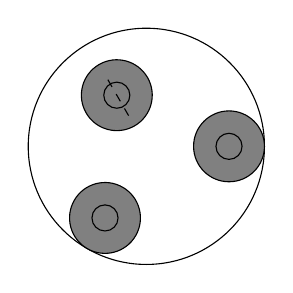
\begin{tikzpicture}[scale=0.5]
		%Circle
			\path node (center) at (0,0) {};
			\draw (center) circle (3);
		%Movable mass
			\draw[rotate=120,fill=gray] (1.5,0) circle (.9) node (moving) [draw,circle]{};
		%Guide
			\draw[dashed,rotate=120] (.9,0) -- (2.1,0);
		%Other masses
			\foreach \i in {1,3}
			{
				\draw[rotate=60-60*\i,fill=gray] (3-.9,0) circle (.9) node[draw,circle]{};
			}
	\end{tikzpicture}
	 & 
	 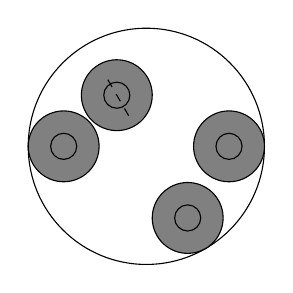
\begin{tikzpicture}[scale=0.5]
		%Circle
			\path node (center) at (0,0) {};
			\draw (center) circle (3);
		%Movable mass
			\draw[rotate=120,fill=gray] (1.5,0) circle (.9) node (moving) [draw,circle]{};
		%Guide
			\draw[dashed,rotate=120] (.9,0) -- (2.1,0);
		%Other masses
			\foreach \i in {1,2,4}
			{
				\draw[rotate=60-60*\i,fill=gray] (3-.9,0) circle (.9) node[draw,circle]{};
			}
	\end{tikzpicture} 
	&
	
	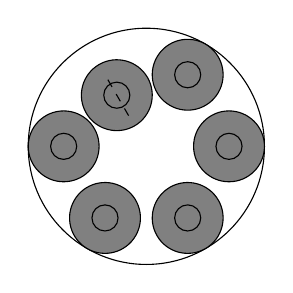
\begin{tikzpicture}[scale=0.5]
		%Circle
			\path node (center) at (0,0) {};
			\draw (center) circle (3);
		%Movable mass
			\draw[rotate=120,fill=gray] (1.5,0) circle (.9) node (moving) [draw,circle]{};
		%Guide
			\draw[dashed,rotate=120] (.9,0) -- (2.1,0);
		%Other masses
			\foreach \i in {1,2,3,4,6}
			{
				\draw[rotate=60-60*\i,fill=gray] (3-.9,0) circle (.9) node[draw,circle]{};
			}
	\end{tikzpicture}
	\\  
	\end{tabular}
	\end{center}
